\section{实验}
\label{sec:exp}

\blue{本文的论点是：好的标记让一个极小的模型便已足够。实验围绕三个问题检验这一论点。建立在三个标记之上的 \sysplus 是否既准确又小巧（第\ref{sec:exp_results}节与第\ref{sec:exp_efficiency}节）？它的每个部分是否都不可或缺——相位通路的各组件（第\ref{sec:exp_ablation}节）以及水平与振幅标记（第\ref{sec:exp_ladder}节）？训练好的模型是否如第\ref{sec:theory}节的统一视角所预测的那样运行（第\ref{sec:exp_theory}节）？第\ref{sec:exp_main}节给出实验设置，第\ref{sec:exp_summary}节回答这三个问题。}

\subsection{\blue{实验设置}}
\label{sec:exp_main}

\blue{代码可在以下地址获取：}\url{\codeurl}。

\fakeparagraph{数据集与设置}
实验在七个广泛使用的长期时间序列预测数据集上进行：
\textit{ETTh1}、
\textit{ETTh2}、
\textit{ETTm1}、
\textit{ETTm2}\footnote{\url{https://github.com/zhouhaoyi/ETDataset}}、
\textit{Weather}\footnote{\url{https://www.bgc-jena.mpg.de/wetter/}}、
\textit{Electricity}\footnote{\url{https://archive.ics.uci.edu/ml/datasets}}、
和 \textit{Traffic}\footnote{\url{https://pems.dot.ca.gov/}}，
涵盖了多样化的真实世界场景。
数据集的详细信息见\blue{电子补充材料}。
参照先前工作~\citep{nie2023patchtst, zhang2023crossformer, huang2025timebase}，ETT 数据集采用 6:2:2 划分，其余数据集采用 7:1:2 划分。
对于 \blue{\sysplus}，我们报告三个随机种子下的平均结果；对于其他基线，我们遵循其官方实现和发布的代码。
我们使用均方误差（MSE）和平均绝对误差（MAE）评估所有被测模型的预测\textbf{精度}，
并从浮点运算数（FLOPs）和参数量（Params）两方面评估\textbf{效率}。

\fakeparagraph{基线与实现细节}
% We evaluate \blue{\sysplus} against eight competitive baselines, encompassing both state-of-the-art Transformer architectures and parameter-efficient forecasting models.
\revised{
我们将 \blue{\sysplus} 与八个有竞争力的基线进行对比，采用标准的无预训练设置，即所有模型直接在特定领域数据集上训练和评估。
这些基线既涵盖最先进的基于 Transformer 的架构，也包括近期的参数高效预测模型。
}
我们将我们的方法与 PatchTST \citeyearpar{nie2023patchtst}、iTransformer \citeyearpar{liu2023itransformer}、Crossformer \citeyearpar{zhang2023crossformer}、FEDformer \citeyearpar{zhou2022fedformer}、TimeBase \citeyearpar{huang2025timebase}、SparseTSF \citeyearpar{lin2024sparsetsf}、FITS \citeyearpar{fits2024} 以及 TimeMixer \citeyearpar{timemixer24} 进行比较。
其中，PatchTST、Crossformer 和 TimeMixer 基于分块；SparseTSF 基于相位；TimeBase 结合了分块与相位两种范式；FITS 和 FEDformer 属于频域方法；iTransformer 则直接对完整序列建模。\blue{此外，FEDformer 和 TimeMixer 还将序列分解为趋势与季节成分。}
对于所有基线，我们采用其官方实现中推荐的配置\revised{，并保持超参数与~\cite{huang2025timebase} 一致。}
模型使用 Adam 优化器优化，学习率固定为 $1 \times 10^{-3}$。
遵循面向效率的工作~\citep{huang2025timebase, lin2024sparsetsf, fits2024} 的设置，输入窗口长度设为 720 个时间步。
更多实现细节见\blue{电子补充材料}。

\blue{
\fakeparagraph{\sysplus 的训练}
\label{sec:ext_setup}
\sysplus 在每个设置上从零开始训练（一个设置指一个数据集与一个预测时域的组合，共 28 个），使用 Huber 损失，最多训练 30 轮，并基于验证损失早停（耐心值为 8），采用三个种子（2021--2023）。选择 Huber 损失是因为其线性尾部可以防止剧烈的水平突变主导梯度，从而稳定训练。所有运行均使用输入长度 $L=720$ 以及上述七个数据集和四个预测时域。标记消融的仅相位变体与相位–水平变体在同一协议下训练，并且 \sysplus 及其相位–水平变体在每个设置和每个种子下都从相同的随机状态构建，因此只要它们共享门控初始化，在初始化时便产生完全相同的预测（第\ref{sec:ext_init}节）。

水平与振幅通路的设计在每数据集一个设置的验证集上确定（ETTh1-96、ETTh2-720、ETTm1-336、ETTm2-96、Weather-192、Electricity-96 与 Traffic-96）。水平解码器在相同秩的三个变体中选择：基于 30 或 90 个池化值的可学习解码器，以及 \equref{eq:branch} 的固定偏移、倾斜与曲率轮廓。门控在逐通道与共享两种形式之间逐数据集选择。选择规则为：只要验证误差相差在 0.5\% 以内，就选择参数最少的变体；只要共享门控与逐通道门控相差在 0.1\% 以内，就选择共享门控。该规则为每个数据集都选定了固定轮廓，并为 ETTh2、ETTm1 和 ETTm2 选定了共享门控。

表\ref{tab:main_results} 中的 \sysplus（即\emph{主表配置}）通过小规模网格搜索逐设置地选择其水平与振幅通路的其余超参数（附录\ref{app:la_config}）。标记消融与第\ref{sec:exp_theory}节的分析在全部 28 个设置上使用同一固定设计，即\emph{协议配置}，其中采用固定轮廓且振幅通路始终启用，从而在所有场合以相同的方式定义。
}

\subsection{\blue{主要结果}}
\label{sec:exp_results}

\begin{table*}[t]
\centering
\caption{
长期预测的主要结果。
\blue{输入长度为 $L=720$，结果为预测时域 $H\in\{96,192,336,720\}$ 上的平均值。}
最好结果以\best{粗体}显示，次好结果以\second{下划线}显示。
\blue{\sysplus 采用主表配置（第\ref{sec:ext_setup}节），结果为三个种子上的平均值。}
}
\label{tab:main_results}
\footnotesize
\setlength{\tabcolsep}{3.6pt}
\begin{tabular}{l|cc|cc|cc|cc|cc|cc|cc}
\hline
\multirow{2}{*}{模型}
& \multicolumn{2}{c|}{ETTh1}
& \multicolumn{2}{c|}{ETTh2}
& \multicolumn{2}{c|}{ETTm1}
& \multicolumn{2}{c|}{ETTm2}
& \multicolumn{2}{c|}{Electricity}
& \multicolumn{2}{c|}{Traffic}
& \multicolumn{2}{c}{Weather} \\
\cline{2-15}
 & MSE & MAE & MSE & MAE & MSE & MAE & MSE & MAE & MSE & MAE & MSE & MAE & MSE & MAE \\
\hline
\blue{\sysplus} & \best{0.401} & \second{0.418} & \second{0.341} & 0.387 & \best{0.351} & \best{0.379} & \best{0.248} & \best{0.313} & \best{0.159} & \best{0.250} & \best{0.392} & \best{0.252} & \best{0.219} & \best{0.256} \\
\hline
PatchTST & 0.420 & 0.439 & 0.344 & 0.390 & \second{0.354} & 0.383 & 0.251 & 0.319 & 0.169 & 0.265 & \second{0.394} & \second{0.266} & \second{0.223} & 0.264 \\
iTransformer & 0.453 & 0.467 & 0.392 & 0.422 & 0.370 & 0.401 & 0.278 & 0.337 & \second{0.165} & 0.263 & 0.406 & 0.290 & 0.233 & 0.273 \\
Crossformer & 0.517 & 0.512 & 1.468 & 0.867 & 0.390 & 0.417 & 0.392 & 0.426 & 0.180 & 0.273 & 0.545 & 0.282 & 0.255 & 0.304 \\
FEDformer & 0.523 & 0.523 & 0.428 & 0.469 & 0.438 & 0.465 & 0.401 & 0.452 & 0.235 & 0.348 & 0.638 & 0.400 & 0.354 & 0.393 \\
TimeBase & \second{0.404} & \best{0.416} & 0.347 & 0.397 & 0.356 & \second{0.380} & \second{0.250} & \second{0.314} & 0.167 & \second{0.258} & 0.418 & 0.278 & 0.227 & \second{0.262} \\
SparseTSF & 0.406 & \second{0.418} & 0.345 & \second{0.383} & 0.362 & 0.383 & 0.252 & 0.316 & 0.168 & 0.263 & 0.413 & 0.280 & 0.243 & 0.285 \\
FITS & 0.419 & 0.435 & \best{0.334} & \best{0.382} & 0.359 & 0.382 & 0.285 & 0.336 & 0.172 & 0.270 & 0.410 & 0.290 & 0.241 & 0.283 \\
TimeMixer & 0.452 & 0.474 & 0.386 & 0.425 & 0.383 & 0.413 & 0.314 & 0.367 & 0.171 & 0.273 & 0.421 & 0.298 & 0.237 & 0.281 \\
\hline
\end{tabular}
\end{table*}

\blue{
表\ref{tab:main_results} 报告了四个预测时域上的平均误差；带标准差的分时域结果见表\ref{tab:la_full}。\sysplus 在七个数据集中的六个上取得最佳平均 MSE，在五个上取得最佳平均 MAE，并且是唯一在全部七个数据集上 MSE 排名第一或第二的模型。唯一的例外是 ETTh2，其中 FITS 领先（0.334），\sysplus 位居第二（0.341）。

两组对比承载了本文的论点。与大模型相比，\sysplus 在每个数据集的两项指标上都更准确，而开销仅为其极小的一部分。在最大的数据集 Traffic 上，它是唯一在两项指标上都比 PatchTST 更准确的模型，将后者的 MAE 降低 5.3\%，而 PatchTST 拥有 7.6M 参数；在 Electricity 上，其 MSE 比第二名 iTransformer 低 3.6\%。将序列分解为趋势与季节成分的 FEDformer 和 TimeMixer 在所有数据集的两项指标上均落后于 \sysplus，这与第\ref{sec:related}节所述的部分覆盖相一致；而基于分块的 PatchTST、Crossformer 和 TimeMixer 在 Electricity 上出现退化——在该数据集上，321 个电表的形状、水平和振幅均因表而异。

与轻量模型相比，\sysplus 在每个数据集上的 MSE 都低于小型跨周期（基于相位的）预测器 TimeBase 和 SparseTSF，在两个传感器网络数据集上领先约 5\% 到 6\%：在 Electricity 上分别领先 4.8\% 和 5.4\%，在 Traffic 上分别领先 6.2\% 和 5.1\%；FITS 在这两个数据集上分别落后 7.6\% 和 4.4\%。与用单一共享线性映射预测每个相位的 SparseTSF 不同，相位通路通过其路由层在相位之间交换信息；在表\ref{tab:ablation_phase} 中每个网络数据集的设置上，移除该层使其在 Electricity 上的 MSE 上升 10.3\%，在 Traffic 上上升 4.6\%（第\ref{sec:exp_ablation}节）。
}

\begin{figure*}[t]
    \centering
    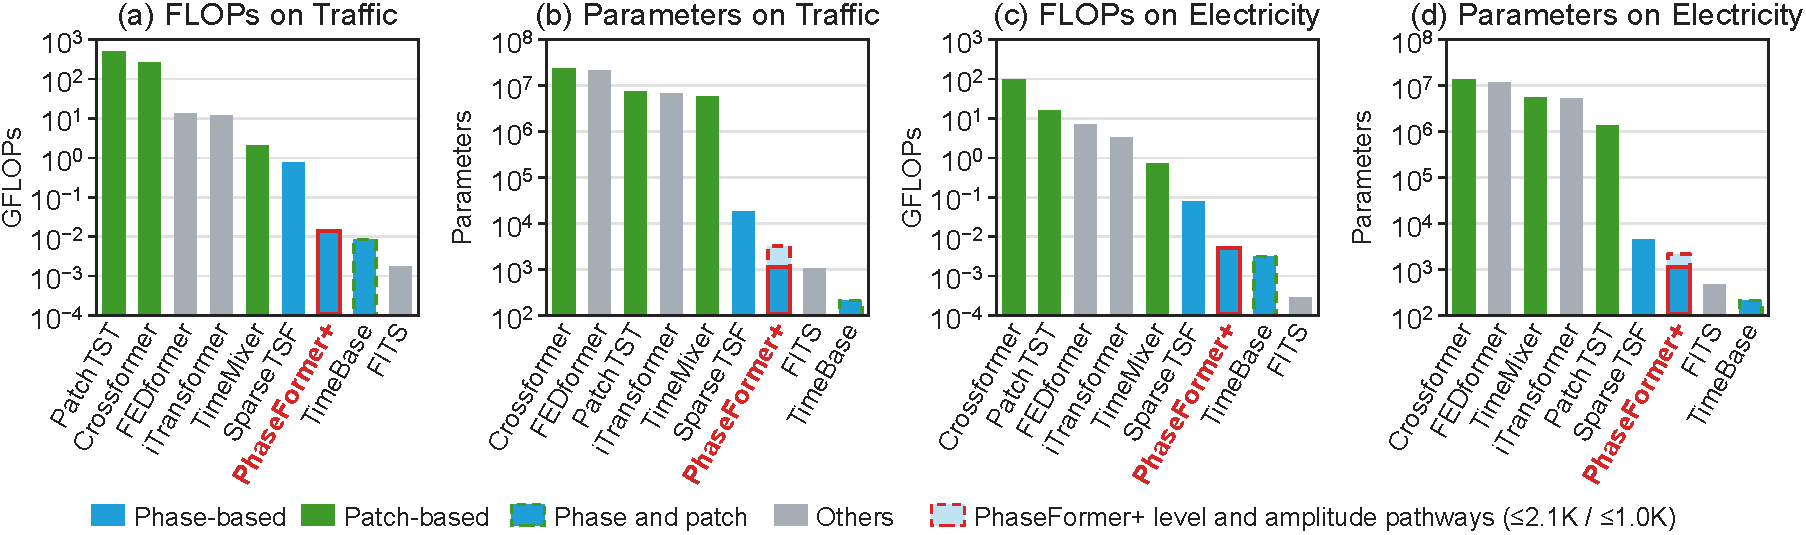
\includegraphics[width=\textwidth]{figures/efficiency_bars.pdf}
    \caption{\blue{\sysplus 与八个基线在 Traffic 和 Electricity 上的单次预测 FLOPs 与参数量，输入长度为 720 步，预测时域为 96（对数坐标）。基于相位的模型为蓝色，基于分块的模型为绿色，结合分块与相位的 TimeBase 为带绿色虚线边框的蓝色，其余模型为灰色。\sysplus 的柱形显示其相位通路；虚线部分加上其水平与振幅通路的参数量，在 Traffic 上至多约 2.1K，在 Electricity 上至多约 1.0K，这部分通路增加的 FLOPs 不足 0.25\%（第\ref{sec:exp_efficiency}节）。}}
    \label{fig:flops_params_visualization}
\end{figure*}

\subsection{\blue{效率}}
\label{sec:exp_efficiency}

我们评估所有模型的计算开销，详细结果见\blue{电子补充材料}。
\figref{fig:flops_params_visualization} 展示了\blue{\sysplus 与八个基线}在 Electricity 和 Traffic \blue{数据集}上的 FLOPs 与参数量。
总体而言，基于相位的模型开销低于基于分块的模型。
在 Traffic 数据集上，\blue{\sysplus 的相位通路}相较 PatchTST 和 Crossformer 将 FLOPs 降低约 99.99\%\blue{，参数量仅约 1.2K}。
这源于相位标记的\blue{低维性}（\secref{sec:mot_stability}）\blue{，使一个小的潜空间和少量路由器即可承载它们。在轻量模型中，\sysplus 在所有数据集上的 MSE 均低于 TimeBase 和 SparseTSF，并在七个数据集中的六个上低于 FITS（第\ref{sec:exp_results}节）。}
\blue{水平与振幅通路保持了这一效率特征。在主表配置的全部 28 个设置中，它们增加的参数量介于 119 到 679 之间。融合门控在共享时共增加两个参数，否则每通道增加两个（Traffic 上为 1{,}724）；它们是唯一规模随传感器数量增长的部分。计入它们后，水平与振幅通路至多增加约 2.1K 参数，最大增量出现在 Traffic 上（第\ref{sec:complexity}节与附录\ref{app:la_config}）。在单块 A800 GPU 上实测（fp32，批大小 32，$L{=}720$），它们使 Traffic 和 Electricity 上相位通路的 FLOPs 增加 $0.09\%$ 到 $0.23\%$：它们的运算——门控、融合、水平标记的周期均值以及两个秩至多为三的映射——相较路由层可以忽略不计。

电子补充材料将 CycleNet 加入对比，后者在 Electricity 上取得了低于 \sysplus 的数据集平均值（补充材料的分时域表中为 0.157，而表\ref{tab:main_results} 中为 0.159）。CycleNet 为每个通道存储一个学习到的周期，在 Electricity 上携带 472K 参数，在 Traffic 上携带 563K 参数，比 \sysplus 高出两个数量级，且这一开销随通道数量增长；\sysplus 则用一条共享通路从自身的相位标记中读取每个通道的形状（逐模型参数量与 FLOPs 对比见电子补充材料）。结合精度结果来看，\sysplus 在七个基准数据集中的六个上取得最佳平均 MSE，同时比 Transformer 基线便宜若干数量级。}

\subsection{\blue{相位通路分析}}
\label{sec:exp_ablation}

\blue{相位通路是三条通路中最大的一条，也是第\ref{sec:exp_ladder}节标记消融的基础。我们单独分析它，即不含水平与振幅通路的情形：其路由器、路由层、相位长度与注意力模式。}

\subsubsection{\blue{路由器数量与跨相位路由}}

\fakeparagraph{改变路由器数量}
我们系统地评估不同路由器数量 $M$ 对模型性能的影响，结果汇总于 \figref{fig:router_number_visualization}。
实验表明，在三个数据集上，模型的预测误差随路由器数量 $M$ 的增加总体呈下降趋势，最终趋于稳定或略有回升。
最佳性能通常在 $M \in \{4,8\}$ 时取得，\blue{远少于相位标记的数量（Electricity 和 Traffic 上为 24）}。
这一观察表明，相位标记张成本质上低维的空间，因此少量路由器便足以有效捕获并表示其底层结构\blue{，这与洞察 2（第\ref{sec:mot_stability}节）一致——根据该洞察，前两个主成分即可解释 Traffic 上相位标记的大部分方差}。
更详细的结果见\blue{电子补充材料}。

\begin{figure*}[t]
    \centering
    % 子图1
    \begin{subfigure}{0.32\textwidth}
        \centering
        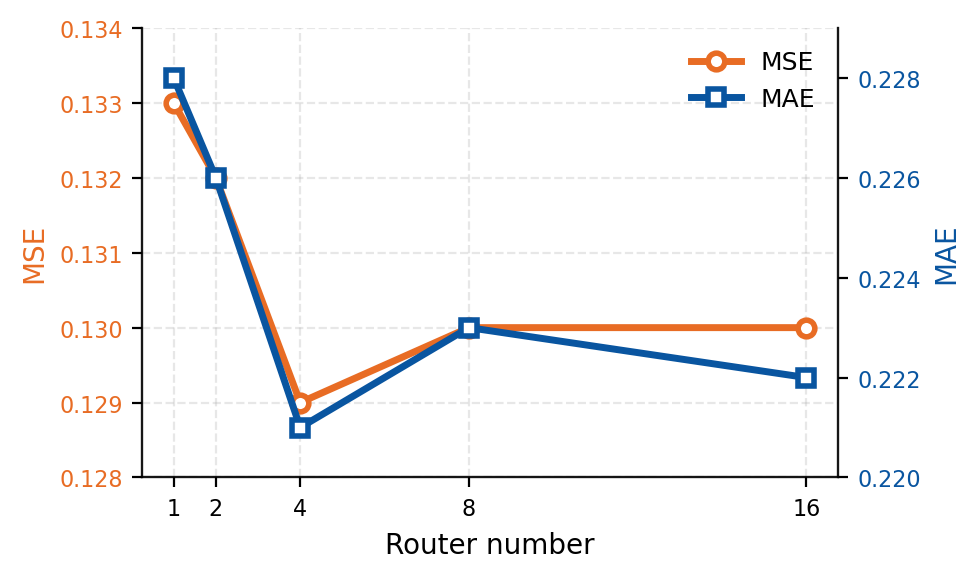
\includegraphics[width=\linewidth]{figures/router_number_effect_electricity_lines.png}
        \caption{Electricity}
        \label{fig:electricity}
    \end{subfigure}
    % 子图2
    \begin{subfigure}{0.32\textwidth}
        \centering
        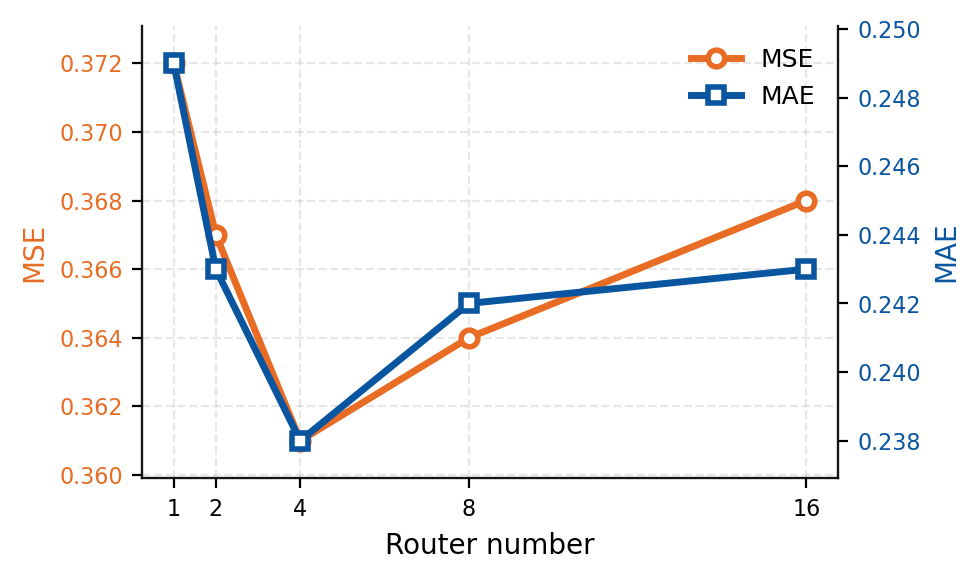
\includegraphics[width=\linewidth]{figures/router_number_effect_traffic_lines.png}
        \caption{Traffic}
        \label{fig:traffic}
    \end{subfigure}
    % 子图3
    \begin{subfigure}{0.32\textwidth}
        \centering
        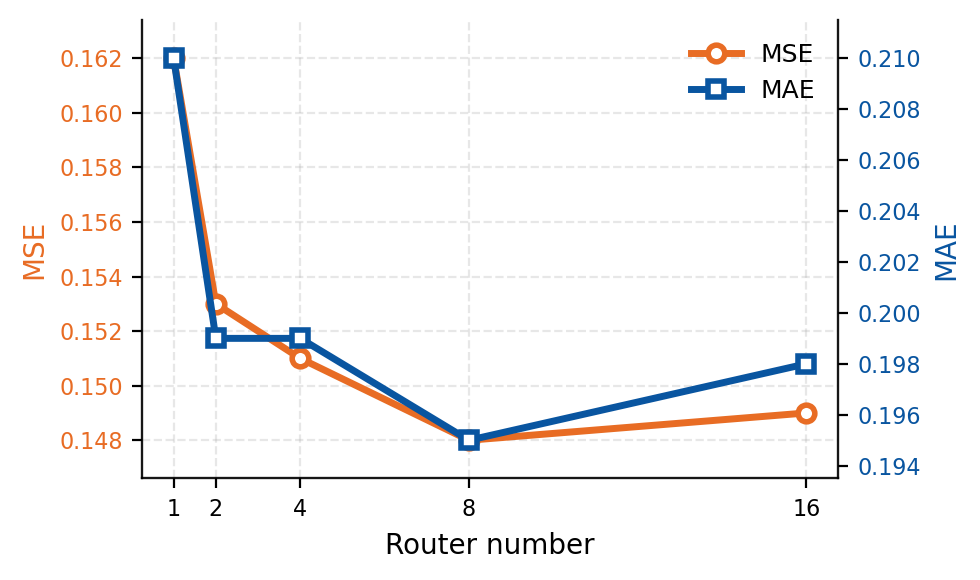
\includegraphics[width=\linewidth]{figures/router_number_effect_weather_lines.png}
        \caption{Weather}
        \label{fig:Weather}
    \end{subfigure}

    \caption{在三个数据集上改变路由器数量 $M$ 对预测性能的影响。}
    \label{fig:router_number_visualization}
\end{figure*}

\begin{table*}[t]
\centering
\caption{\blue{相位通路跨相位路由层的消融。}每个单元格报告 MSE、MAE 和 FLOPs。所有指标均为越低越好。FLOPs 以百万（MFLOPs）为单位报告。最好结果以\best{粗体}标出，次好结果以\second{下划线}标出。}
\label{tab:ablation_phase}
\footnotesize
\begin{tabular}{c|ccc|ccc|ccc|ccc}
\hline
\multirow{2}{*}{数据集}
& \multicolumn{3}{c|}{\textbf{路由}}
& \multicolumn{3}{c|}{\textbf{采用全注意力}}
& \multicolumn{3}{c|}{\textbf{采用线性混合}}
& \multicolumn{3}{c}{\textbf{去除路由}} \\
\cline{2-13}
& MSE & MAE & FLOPs
& MSE & MAE & FLOPs
& MSE & MAE & FLOPs
& MSE & MAE & FLOPs \\
\hline
Weather
& \best{0.1503} & \best{0.1971} & 3.119
& \second{0.1527} & \second{0.2005} & 3.202
& 0.1700 & 0.2226 & \second{0.920}
& 0.1907 & 0.2406 & \best{0.783} \\
\hline
Electricity
& \best{0.1290} & \best{0.2209} & 42.213
& \second{0.1295} & \second{0.2217} & 48.951
& 0.1403 & 0.2334 & \second{14.068}
& 0.1423 & 0.2365 & \best{11.972 } \\
\hline
Traffic
& \best{0.3721} & \best{0.2475} & 113.356
& \second{0.3791} & \second{0.2513} & 131.452
& 0.3842 & 0.2532 & \second{37.776}
& 0.3892 & 0.2584 & \best{32.149}  \\
\hline
\end{tabular}
\end{table*}

\fakeparagraph{跨相位路由的有效性}
为评估跨相位路由层的贡献，我们比较\blue{相位通路}的四个变体：
\textbf{路由}，采用跨相位路由层；
\textbf{采用全注意力}，用完整注意力机制替换跨相位路由层；
\textbf{采用线性混合}，用线性层替换跨相位路由层；
以及 \textbf{去除路由}，直接将每个相位投影到其自身的未来。
其余实验设置在这些变体之间保持完全一致。

如 \tabref{tab:ablation_phase} 所总结，\blue{路由}一致优于 \textbf{采用线性混合} 和 \textbf{去除路由}，表明显式的跨相位路由对建模周期性动态至关重要。此外，\blue{路由}不仅\blue{计算量}更小，预测误差也低于 \textbf{采用全注意力}，说明路由层兼具高效与有效。我们将这些增益归因于在低维相位标记空间中运算，该空间集中了信息丰富的交互并降低了开销。

\revised{
\subsubsection{对相位长度的敏感性}
\label{sec:phase_length}

\begin{table}[t]
\centering
\begin{tabular}{ccc}
\hline
\textbf{相位长度} & \textbf{MSE} & \textbf{MAE} \\
\hline
24 & 0.3619 & 0.2384 \\
12 & 0.3960 & 0.2765 \\
8  & 0.4032 & 0.2801 \\
28 & 0.4063 & 0.2753 \\
21 & 0.4184 & 0.2970 \\
\hline
\end{tabular}
\caption{Traffic 数据集上不同相位长度下预测性能的比较（\blue{$L=720$，$H=96$}）。}
\label{tab:phase_length}
\end{table}
\blue{\sysplus} 通过频域分析自动确定相位长度（见\blue{电子补充材料}），直接从数据中提取显著的周期成分。
为评估其对相位长度的敏感性，我们在 Traffic 数据集上开展实验。其频谱包含若干清晰的周期成分（见 \figref{fig:spectrum_traffic}）。我们基于谱幅值选出前五个候选相位长度，并运行\blue{相位通路}进行预测。结果如 \tabref{tab:phase_length} 所示。

\begin{figure}[t]
    \centering
    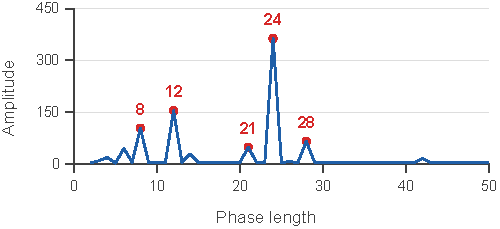
\includegraphics[width=\linewidth]{figures/spectrum_traffic.pdf}
    \caption{在 Traffic 数据集上计算的频谱。前五个相位长度为 24、12、8、28、21。}
    \label{fig:spectrum_traffic}
\end{figure}

实验表明，相位长度为 24 时模型表现最佳，对应主导谱成分。\blue{五个候选的 MSE 恰好按其谱幅值的顺序递增（\figref{fig:spectrum_traffic}），因此最强的谱成分也是最准确的相位长度。}
这些发现表明，\blue{相位通路}有效捕获了数据集的主要周期结构。
}

\subsubsection{案例分析}
\label{sec:exp_case}
我们从 Traffic 数据集中选取一个样本，包含长度为 720 的输入序列和长度为 96 的输出序列（共 816 个时间步）。
将输入序列送入\blue{相位通路}，我们记录第一个跨相位路由层在聚合（Phase$\rightarrow$Router）与分发（Router$\rightarrow$Phase）两个阶段的注意力权重矩阵。
如 \figref{fig:sender} 与 \figref{fig:receiver} 所示，两种注意力模式都呈现清晰的局部相似性：相邻相位往往被分配到相同的路由器，并从相似的路由器接收注意力。
这表明路由机制捕获了时间上连贯的相位关系。
同时，注意力权重显示某些相位具有相似的注意力模式。
为进一步分析，我们聚焦三个具有不同注意力模式的相位，并在 \figref{fig:traffic_data_visualization} 中将其\blue{可视化}。
这些相位表现出不同的时间行为：相位 5 在较长时域上保持相对稳定，而相位 9 和相位 1 都呈现明显的 7 天周期性，但趋势相反。
这些相位标记的不同模式表明，路由器结构不仅能区分相位标记，还能有效建模其\blue{每周模式与漂移}。
\blue{总的来说，这些分析说明了相位通路为何可以很小：相位标记是低维的，少量路由器即已足够；路由比完整注意力和无交换都更准确，且 FLOPs 至多比完整注意力少 14\%；主导周期也是最准确的相位长度。还有一点预示了标记消融：路由器曲线在少量路由器处便趋于平缓，因此相位通路中新增的容量不再带来收益，而仅有 105 个参数的水平通路仍能将 Weather 上的 MSE 改善 2.7\%（第\ref{sec:exp_ladder}节）。}


\begin{figure*}[t]
  \centering
  \begin{subfigure}{0.24\linewidth}
    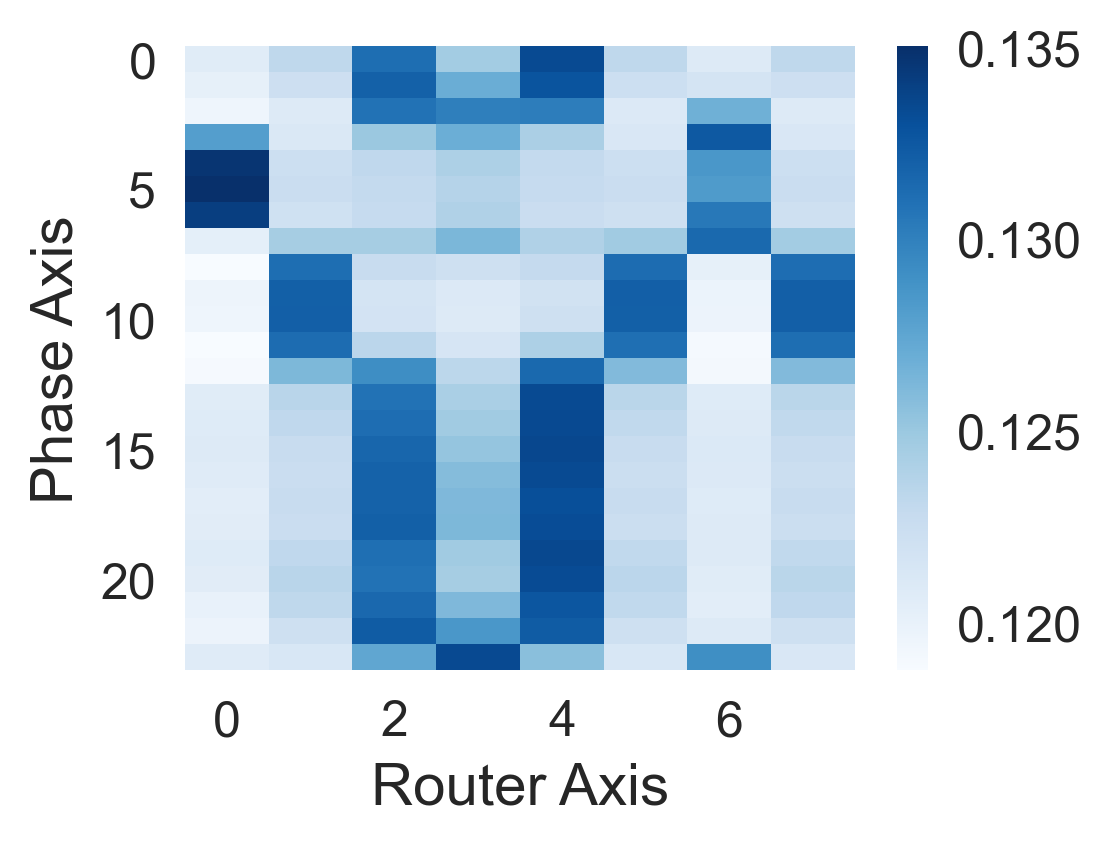
\includegraphics[width=\linewidth]{figures/attention_layer_0_sender_var4.png}
    \caption{聚合权重}
    \label{fig:sender}
  \end{subfigure}%
  \hfill
  \begin{subfigure}{0.24\linewidth}
    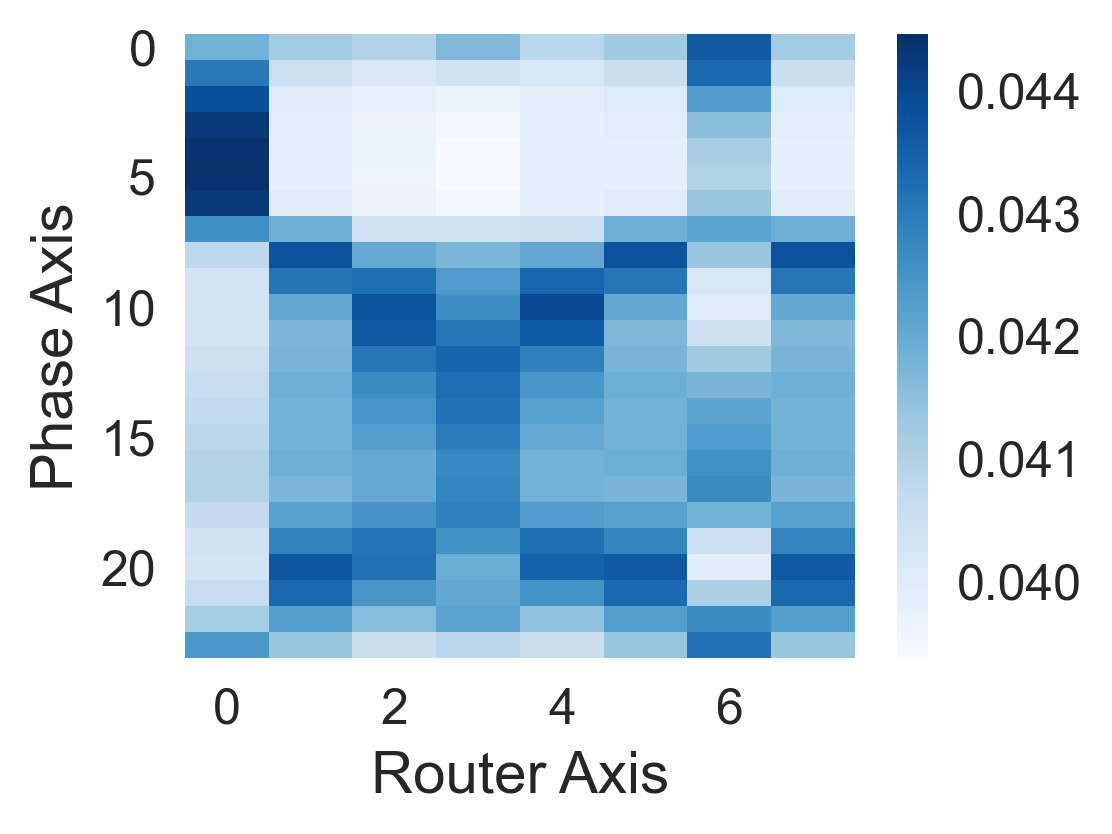
\includegraphics[width=\linewidth]{figures/attention_layer_0_receiver_var4.png}
    \caption{分发权重}
    \label{fig:receiver}
  \end{subfigure}
  \hfill
  \begin{subfigure}{0.48\linewidth}
    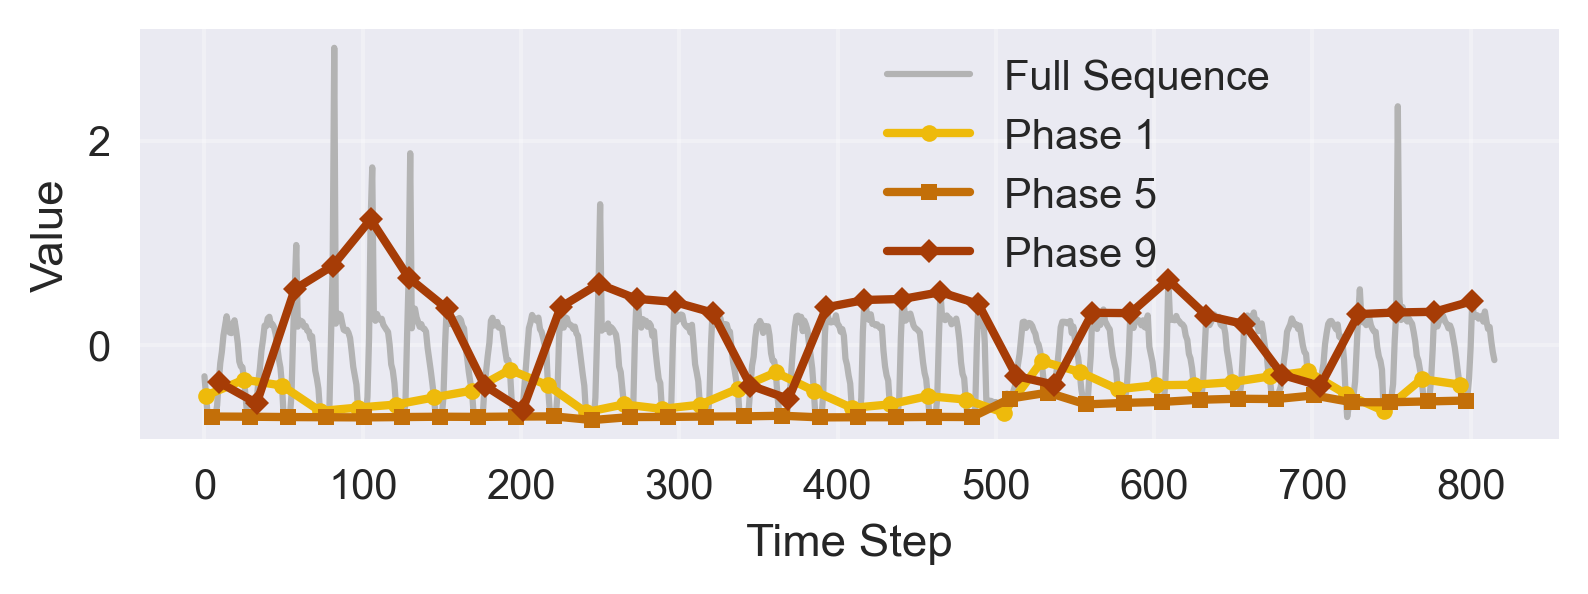
\includegraphics[width=\linewidth]{figures/sequence_with_phase_curves_sample_0_feature_0.png}
    \caption{三个选定相位标记的可视化}
    \label{fig:traffic_data_visualization}
  \end{subfigure}%
  \caption{Traffic 数据集一个样本的案例分析。
  (a) 相位到路由器聚合阶段的注意力权重矩阵。
  (b) 路由器到相位分发阶段的注意力权重矩阵。
  两个矩阵都刻画了 8 个路由器与 24 个输入相位之间的关联。
  (c) 三个代表性相位（1、5 和 9）的可视化，每个相位都对应一种与路由器交互的独特注意力模式。}
  \label{fig:case_study_wrap_all}
\end{figure*}

\blue{
\subsection{每个标记都不可或缺}
\label{sec:exp_ladder}

\begin{table*}[t]
\blue{
\centering
\caption{标记消融：\sysplus 逐个添加标记构建。测试 MSE/MAE 为四个预测时域与三个种子上的平均值，所有变体在同一协议下训练（协议配置，第\ref{sec:ext_setup}节）。仅相位：仅相位变体；相位 + 水平：相位–水平变体；\sysplus（关闭振幅）：关闭振幅通路后的训练好的 \sysplus。粗体：前三列中的最佳值。正文中的相对差异基于未取整的平均值计算。}
\label{tab:ladder}
\footnotesize
\setlength{\tabcolsep}{6pt}
\begin{tabular}{lcccccccc}
\toprule
数据集 & \multicolumn{2}{c}{仅相位} & \multicolumn{2}{c}{相位 + 水平} & \multicolumn{2}{c}{\sysplus} & \multicolumn{2}{c}{\begin{tabular}[c]{@{}c@{}}\sysplus\\（关闭振幅）\end{tabular}} \\
\cmidrule(lr){2-3}\cmidrule(lr){4-5}\cmidrule(lr){6-7}\cmidrule(lr){8-9}
 & MSE & MAE & MSE & MAE & MSE & MAE & MSE & MAE \\
\midrule
ETTh1 & 0.408 & \textbf{0.419} & 0.412 & 0.425 & \textbf{0.405} & 0.421 & 0.414 & 0.429 \\
ETTh2 & 0.354 & 0.396 & \textbf{0.347} & \textbf{0.393} & 0.348 & \textbf{0.393} & 0.352 & 0.396 \\
ETTm1 & \textbf{0.352} & \textbf{0.377} & 0.354 & 0.380 & 0.353 & 0.380 & 0.355 & 0.381 \\
ETTm2 & 0.258 & 0.319 & \textbf{0.253} & \textbf{0.315} & \textbf{0.253} & \textbf{0.315} & 0.257 & 0.318 \\
Weather & 0.227 & 0.262 & 0.221 & \textbf{0.257} & \textbf{0.220} & \textbf{0.257} & 0.220 & 0.257 \\
Electricity & 0.161 & \textbf{0.251} & \textbf{0.160} & \textbf{0.251} & \textbf{0.160} & \textbf{0.251} & 0.162 & 0.254 \\
Traffic & \textbf{0.392} & \textbf{0.248} & 0.395 & 0.251 & 0.393 & 0.252 & 0.400 & 0.256 \\
\bottomrule
\end{tabular}
}
\end{table*}

表\ref{tab:ladder} 在协议配置下、全部 28 个设置、三个种子上逐个添加标记构建 \sysplus：先是仅相位变体（第\ref{sec:ext_setup}节），然后是水平标记，再是振幅标记；其最后一列为在训练好的 \sysplus 上关闭振幅通路。在同一协议下，\sysplus 在七个数据集平均值中的五个上优于其仅相位变体，幅度介于 0.4\% 到 3.3\% 之间；在 ETTm1 和 Traffic 上与其相差不超过 0.3\%，参数开销约为 130--170（不含融合门控）。包络同时预示了这一结果的两个方面。四个最大的增益恰好落在四个包络生效的数据集上：Weather、ETTm2 和 ETTh2 上的水平包络，以及 ETTh1 上的振幅包络（表\ref{tab:envelope}）。在 ETTm1、Electricity 和 Traffic 上，落在任一包络之外的测试窗口都不超过 3.5\%，误差变化至多 0.4\%，正如理论所预测。在主表配置下，\sysplus 在 ETTh2、ETTm2 和 Weather 的每个预测时域上都优于仅相位变体，且优势超过一个种子标准差（表\ref{tab:la_full}）。

\fakeparagraph{水平标记}
水平标记恰好在水平包络生效之处取得增益，无论在仅相位变体上还是在 \sysplus 上皆如此（第\ref{sec:exp_envelopes}节）。在 ETTh2、ETTm2 和 Weather 上，分别有 7.8\% 到 9.7\% 的测试窗口落在仅相位变体的包络之外，12\% 到 21\% 落在 \sysplus 的包络之外，水平标记将 MSE 分别改善 2.0\%、1.8\% 和 2.7\%；在其余四个数据集上（落在包络之外的窗口至多 3.5\%），它对误差的改变至多 1.0\%。

\fakeparagraph{振幅标记}
振幅标记补充了水平标记所无法提供的能力。ETTh1 是唯一一个振幅包络生效而水平包络几乎不生效的数据集（窗口占比 14.8\% 对 2.5\%，表\ref{tab:envelope}）；在此，仅添加水平标记会使误差增加 1.0\%，振幅标记带来了恢复，\sysplus 最终比仅相位变体低 0.7\%。在训练好的模型上关闭振幅通路会消除全部增益（0.414 对 0.405）。在全部 28 个设置中，振幅通路在 27 个设置上改善了其所属模型。

\fakeparagraph{弱耦合与强耦合}
在耦合最弱的两个基准数据集 ETTh2 和 ETTm2 上（第\ref{sec:mot_changes}节），增益由水平标记贡献，而振幅通路在 \sysplus 内部仍在发挥作用：关闭它会使 MSE 从 0.348 升至 0.352、从 0.253 升至 0.257。在耦合如此弱的情况下，ETTh2 上超出振幅包络的 31.8\% 窗口，其超出量来自窗口自身的形状 $\Omega_0$，而非水平。在耦合最强的基准数据集 Traffic 上，尽管没有窗口超出包络，振幅通路仍改善了其所属模型（0.393 对关闭时的 0.400）；这一增益将 $q$ 的静态逐通道修正（第\ref{sec:exp_mechanism}节）与依赖水平的部分结合起来，下文的分层分析将其揭示出来。

\fakeparagraph{增益出现之处}
如果振幅通路承载的是跟随水平的振幅，那么 \sysplus 相对其相位–水平变体的逐窗口增益应随水平需求增长。按 $|\Lambda|$ 的五分位数对逐窗口测试增益分层的结果支持这一点。在全部 28 个设置中，最高五分位的 MSE 降幅比最低五分位多 $0.002$；在 \sysplus 平均而言有所改善的大多数设置上，最高五分位的平均增益超过最低五分位，其中最强的设置从低到高逐层上升（Traffic-$96$：各五分位从 $+0.0002$ 到 $+0.0033$；ETTh1-$192$：$-0.0033$ 到 $+0.0052$；Weather-$96$：$-0.0031$ 到 $+0.0080$）。因此，振幅通路在水平变化最大的窗口上增益最大。
}

\blue{
\subsection{验证统一视角}
\label{sec:exp_theory}

第\ref{sec:theory}节分三步展开论证，每一步都可以在训练好的模型上检验。必要性：包络在每个训练好的模型上都成立，并在数据的需求超出它们之处生效；此时水平通路接管水平，而振幅通路不改变任何周期均值，因此它无法替代水平通路（第\ref{sec:exp_envelopes}节与第\ref{sec:exp_mechanism}节）。形式：振幅通路的增益随数据中由水平驱动的振幅而增长，并读取水平（第\ref{sec:exp_mechanism}节）。充分性：三个固定轮廓、105 个参数，与可学习解码器相比几乎没有损失（第\ref{sec:exp_capacity}节）。

\subsubsection{包络与分工}
\label{sec:exp_envelopes}

定理\ref{thm:level_envelope}与定理\ref{thm:amplitude}的常数是权重的函数，因此可以从每个训练好的模型中读出，而需求是数据的函数。表\ref{tab:envelope} 针对训练好的 \sysplus 模型（在四个预测时域上取平均）报告了这两组量，以及每个测试窗口的水平需求 $\Lambda$ 与振幅需求 $\Omega$。

\begin{table}[t]
\blue{
\centering
\caption{训练好的 \sysplus 模型相位通路的包络（协议配置；预测时域上的平均值；振幅通路已关闭）。$C_1$、$B_\varphi$：水平包络与振幅包络的半宽，从权重中读出；$g_s$：形状门控；$\mathcal I_\varphi$ 之外：水平需求 $\Lambda$ 落在水平包络之外的测试窗口占比；下界/MSE：误差下界~\equref{eq:level_floor} 占测试 MSE 的比例；$\Omega$ 超包络：振幅需求超过 $(1-g_s)B_\varphi$ 的窗口占比。}
\label{tab:envelope}
\footnotesize
\setlength{\tabcolsep}{2.6pt}
\begin{tabular}{lcccccc}
\toprule
数据集 & $C_1$ & $B_\varphi$ & $g_s$ & $\mathcal I_\varphi$ 之外 & 下界/MSE & $\Omega$ 超包络 \\
\midrule
ETTh1 & 1.35 & 1.37 & 0.23 & 2.5\% & 0.08\% & 14.8\% \\
ETTh2 & 1.07 & 1.08 & 0.25 & 19.4\% & 5.0\% & 31.8\% \\
ETTm1 & 1.86 & 1.99 & 0.35 & 3.5\% & 0.27\% & 2.2\% \\
ETTm2 & 1.39 & 1.47 & 0.26 & 12.5\% & 10.6\% & 5.7\% \\
Weather & 1.41 & 1.61 & 0.68 & 20.7\% & 11.6\% & 27.6\% \\
Electricity & 3.80 & 3.81 & 0.27 & 0.1\% & 0.5\% & 0.2\% \\
Traffic & 5.23 & 5.25 & 0.21 & 0.0\% & 0.0\% & 0.0\% \\
\bottomrule
\end{tabular}
}
\end{table}

\fakeparagraph{包络成立}水平包络严格按所述成立：在全部 84 个训练好的模型（28 个设置、三个种子）中，相位预测的实测水平从未离开 $\mathcal I_\varphi$，$|\lev(F)-c_0|/C_1$ 的最大观测值为 $0.74$，因此下文给出的下界是保守的。

\fakeparagraph{包络在理论预测之处生效}在包络生效之处，其生效方式与理论预测一致。在 ETTh2、Weather 和 ETTm2 上，有 12\% 到 21\% 的测试窗口的水平需求落在区间之外，下界占测试 MSE 的 5.0\% 到 11.6\%；并且在 ETTh2 和 Weather 上，包络外窗口的占比与区间的收紧程度都随预测时域增长（ETTh2：在 $H=96$ 到 $H=720$ 之间，$C_1$ 从 1.27 降到 0.85，包络外占比从 15\% 升到 27\%；Weather：从 1.86 降到 0.96，从 10\% 升到 34\%）。在两个传感器网络数据集上，训练好的模型的相位通路形成了几乎没有任何测试窗口能越出的宽包络。它们的半宽（$C_1$ 介于 3.8 与 5.2 之间）低于一致跟踪最后一个周期水平所需的 5.39（第\ref{sec:theory_level}节），但测试窗口的水平需求更小，下界至多占测试 MSE 的 0.5\%。因此，包络在这些数据集上几乎没有给相位通路带来损失，添加水平与振幅标记在这两个数据集上对误差的改变不足 1\%（第\ref{sec:exp_ladder}节）。

\fakeparagraph{分工遵循包络}水平门控在每个数据集上取得相近的份额（$g_\ell$ 平均在 0.20 到 0.26 之间），但水平通路如何使用其份额取决于包络是否生效：在包络较窄（$C_1\le1.86$）的四个 ETT 数据集上，水平通路的水平预测与窗口水平需求的相关系数在 $0.40$ 到 $0.44$ 之间；而在包络较宽的 Electricity 和 Traffic 上，分别为 $0.03$ 和 $-0.01$。水平通路在相位通路无法跟踪水平之处跟踪水平，正如定理\ref{thm:complement}(b) 所预测。

以同样方式考察 84 个训练好的仅相位变体可以看出，这一模式是数据的属性，在没有水平与振幅标记时同样存在。它们的预测水平同样从未离开包络（最大观测利用率为 $0.87$），且水平包络在同样的三个数据集上生效：在 ETTh2、ETTm2 和 Weather 上，有 7.8\% 到 9.7\% 的测试窗口落在包络之外，下界占测试 MSE 的 1.7\% 到 4.1\%，而在其余四个数据集上分别至多只有 3.5\% 和 0.6\%。与水平通路共同训练时，\sysplus 的相位通路在这三个数据集上收窄了其包络（$C_1$ 从 1.72--2.16 之间降到 1.07--1.41 之间），在 ETTh1 和 ETTm1 上的变化不超过 0.1，并在两个传感器网络数据集上加宽了包络：在水平包络生效之处，它把水平留给水平通路，这正是定理\ref{thm:complement}(b) 的分工。

\subsubsection{振幅通路}
\label{sec:exp_mechanism}

\fakeparagraph{合成乘性序列}
我们首先在真值已知的场景下检验定理\ref{thm:amplitude}。我们按 \equref{eq:mult_model} 生成具有随机游走水平、正弦日轮廓和耦合 $\alpha\in\{0,0.25,0.5\}$ 的七通道序列，并从相同初始化训练 \sysplus 及其相位–水平变体（两个种子、30 轮）。无耦合（$\alpha=0$）时，振幅通路无事可承，两个模型难分伯仲：\sysplus 的验证 MSE 变化为 $-0.28\%$。有耦合时，\sysplus 在 $\alpha=0.25$ 下将验证 MSE 降低 $3.3\%$，在 $\alpha=0.5$ 下降低 $4.8\%$，且对两个种子均是如此。增益恰好在数据包含跟随水平的振幅时出现，并随耦合增强而增长，正如定理\ref{thm:amplitude}(b) 中需求的形式与命题\ref{prop:modulation}(b) 的构造所蕴含的那样。

\fakeparagraph{周期均值不变性}
命题\ref{prop:modulation}(a) 是精确的恒等式，因此我们在每个训练好的 \sysplus 上对其进行验证。在双精度下开关振幅通路，对相位预测的每个未来周期均值的绝对改变至多为 $8.9\times10^{-16}$，而容差为相对于预测尺度的 $7\times10^{-9}$，而对单个相位预测的改变最多可达 $1.8$ 个窗口标准差。全部 84 个训练好的模型（28 个设置、三个种子）均通过验证。

\fakeparagraph{振幅通路读取水平}
命题\ref{prop:modulation}(b) 预测振幅通路会读取水平：其构造 $q=\alpha_w\hat\Lambda\,\one_d$（其中 $\hat\Lambda$ 为水平通路的水平预测）以因子 $1+\alpha_w\hat\Lambda$ 缩放相位振幅。训练好的模型证实了这一点，在 $H=96$ 时最为清晰；在读取水平较弱之处，振幅通路充当静态的逐通道振幅修正，这由 $q$ 的均匀分量提供（第\ref{sec:theory_amplitude}节）。我们逐通道计算 $q$ 沿 $\one_d$ 方向的分量与窗口水平需求 $\Lambda$ 的相关系数；合并通道会把 $q$ 中由水平驱动的部分与其依赖通道的静态尺度混在一起。在 $H=96$ 时，逐通道平均相关系数在 Weather 上为 $0.46$（86\% 的通道）、在 Electricity 上为 $0.30$（全部 166 个显著通道同号）、在 ETTh2 上为 $0.54$（每个通道都超过 $0.3$）；在七个数据集上按预测时域平均后介于 $0.12$ 与 $0.37$ 之间。学习到的耦合符号在每个设置内保持一致——Weather-$96$ 的显著通道与 Electricity-$96$ 的符号相反——这是构造所允许的，因为 $\alpha_w$ 是学习得到的。

在 ETTm1-$96$ 和 ETTm2-$96$ 上相关系数较低（$0.27$ 和 $0.02$）：在这两个设置上，振幅通路主要充当静态修正。另外两个观察也与构造一致：$q$ 与振幅需求 $\Omega$ 本身仅有弱相关（各处逐通道平均相关系数均低于 $0.20$），因此它跟随的是水平而非振幅；$q$ 的静态部分是一个逐通道振幅修正，其移除可以解释表\ref{tab:ladder} 中关闭振幅列在七个数据集中六个上的退化。

\subsubsection{水平通路的容量}
\label{sec:exp_capacity}

定理\ref{thm:complement}(a) 预测，在标准季节模型下，相位通路无法企及的水平通过少数固定时域轮廓进入，因此轮廓预先固定的水平通路与学习这些轮廓的水平通路相比应当毫无损失。第\ref{sec:ext_setup}节的选择实验提供了直接检验。在相同秩下，三种解码器的参数量差异悬殊：可学习解码器分别有 477 和 657 个参数，是固定轮廓 105 个参数的四到七倍。然而它们的按设置归一化的验证误差——在七个数据集与两种门控变体上平均——仅相差 0.13\%：相对于每个设置的最佳变体，基于 90 个池化值的解码器为 1.0102，基于 30 个池化值的解码器为 1.0107，固定轮廓为 1.0115。固定轮廓落在与最佳解码器相差 0.5\% 的平局范围内，并因其最小而入选。因此，限制在偏移、倾斜与曲率轮廓张成空间中的水平通路，与能学习任意时域轮廓的水平通路相比几乎没有损失，正如定理\ref{thm:complement}(a) 所预测；这三个轮廓已经足够：即便在主表配置中，28 个设置中也有 24 个保留它们（附录\ref{app:la_config}）。

}

\blue{
\subsection{总结}
\label{sec:exp_summary}

实验回答了本节的三个问题。其一，\sysplus 既准确又小巧：它在七个基准数据集中的六个上取得最佳平均 MSE，并在全部七个上排名第一或第二。在最大的基准数据集 Traffic 上，其相位通路仅需约 1.2K 参数，即可将 PatchTST 和 Crossformer 的 FLOPs 降低约 99.99\%，而水平与振幅通路至多增加约 2.1K 参数。其二，每个部分都不可或缺：在相位通路中，跨相位路由比完整注意力和无交换都更准确，且只需少量路由器；在统一协议下逐个添加标记构建时，\sysplus 恰在包络预测之处获得增益，其四个最大的增益正落在四个包络生效的数据集上。其三，训练好的模型的表现与统一视角的预测一致：水平包络在每个模型上都成立，并且恰好在水平标记增益最大的三个数据集上生效；振幅通路精确保持每个周期均值并读取水平；三个固定轮廓足以支撑水平通路。因此，预测周期性传感器数据流并不需要当前模型那样的复杂度：有了覆盖形状、水平与振幅的标记，一个只有几千个参数的模型便已足够。
}
